\chapter{绪论}

\section{研究背景与意义}

人类大脑是自然界已知最复杂的智能系统，在感知、认知、情绪加工及行为决策等多层次任务中展现出卓越的效率与灵活性\citep{hassabis2017neuroscience}。理解大脑如何在复杂环境中处理信息、形成认知并驱动行为，是神经科学、认知科学以及人工智能领域长期关注的核心问题。随着神经科学与计算科学的协同发展，利用计算模型解析神经活动，并逆向重建其对应的认知状态或行为意图，已成为脑科学与人工智能交叉融合的重要方向\citep{haynes2006decoding}。神经信号解码作为连接生物智能与人工智能的关键桥梁\citep{wolpaw2007brain}，对于揭示大脑信息处理机制及推动新一代类脑人工智能系统发展具有重要意义\citep{makeig2012evolving}。

近年来，脑机接口（Brain–Computer Interface, BCI）\citep{gao2021interface}技术的发展进一步推动了神经信号解码研究的深入。BCI系统通过直接采集并解析大脑神经活动，实现人类与外部设备之间的直接交互，从而为运动功能障碍患者提供辅助控制能力，并拓展了人机交互的技术路径\citep{kawala2021summary,gao2025brain}。非侵入式BCI因其安全性高、成本低和易于推广等优势，在临床康复、人机交互、情绪监测等领域展现出广阔的应用前景。常见的非侵入式神经信号主要包括脑电图（Electroencephalography, EEG）\citep{al2018review}、脑磁图（Magnetoencephalography, MEG）\citep{mellinger2007meg, hajipour2012selection}、功能性近红外光谱（functional Near-Infrared Spectroscopy, fNIRS）\citep{shin2020performance, lim2020unified}以及功能性磁共振成像（functional Magnetic Resonance Imaging, fMRI）\citep{yoo2004brain, weiskopf2003physiological}等。这些神经成像技术从不同角度刻画大脑活动，为研究复杂脑功能提供了重要数据来源。然而，由于脑信号本身具有高噪声、强非线性以及显著个体差异等特点，如何从复杂的神经数据中准确、稳定地解码人类意图与认知状态，仍然是脑机接口研究领域面临的关键挑战。

\section{国内外研究现状}

\subsection{EEG单模态解码的研究现状}

EEG能够以毫秒级时间分辨率记录大脑皮层神经元群体的电活动变化，是当前非侵入式BCI研究中最常用的神经信号之一。由于其采集设备成本较低、操作相对简便，并且能够直接反映神经电活动的动态变化，EEG被广泛应用于运动想象识别、认知状态监测以及情绪识别等多种BCI任务中\citep{al2018review,sitaram2009hemodynamic}。随着BCI研究的不断发展，如何从复杂且高噪声的EEG信号中提取具有判别力的神经特征并实现可靠解码，成为该领域的重要研究问题。

通常，EEG信号解码过程可以划分为三个关键步骤：预处理、特征提取和分类，如图~\ref{fig:figure1}~所示。预处理阶段用于去除噪声与伪迹，为后续分析提供更稳定的信号基础；特征提取阶段将原始脑电信号转换为具有判别能力的紧凑表示；分类阶段则根据提取的特征识别不同的脑状态或行为意图。

\begin{figure}[htbp]
    \centering
    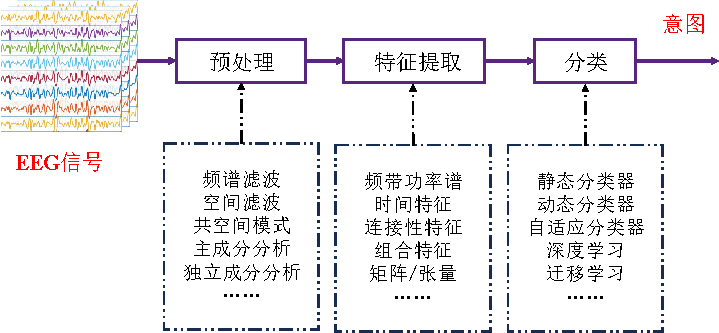
\includegraphics[scale=1]{pic/图片0-crop.pdf}
    \caption{EEG信号解码基本流程}
    \label{fig:figure1}
\end{figure}

\subsection{研究现状2}
 
\subsection{研究现状3}

\subsection{现有研究的不足与挑战}

综上所述，尽管已有研究取得了一定进展，但由于××××，现有方法仍面临以下共性挑战：

\section{研究内容与章节安排}

\subsection{研究内容}

针对现有研究的不足与挑战，本文围绕……，系统开展方法研究，构建……，整体研究思路如图~\ref{fig:figure0}~所示。具体研究内容包括：

\begin{figure}[H]
    \centering
    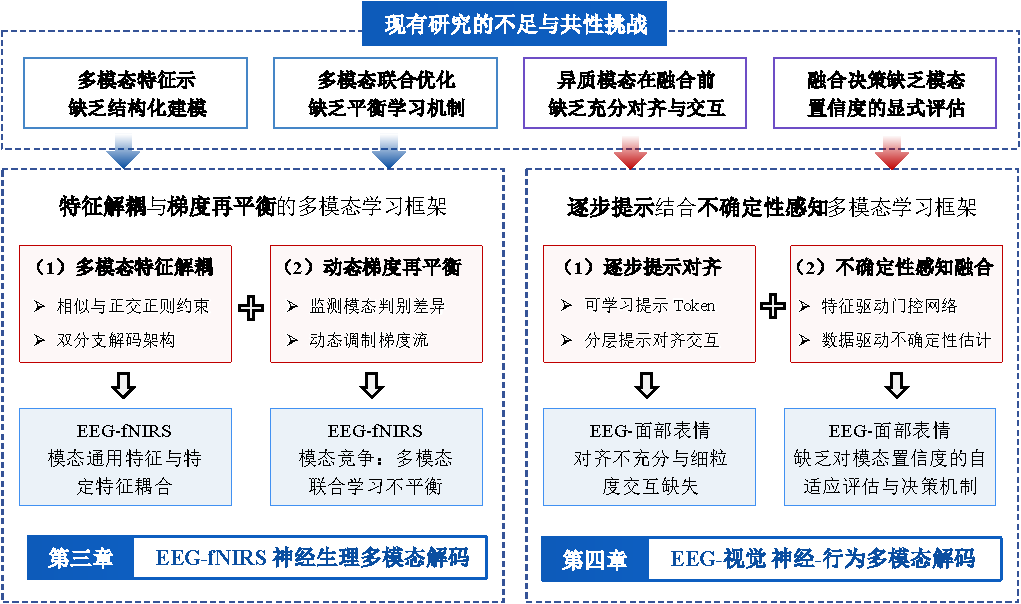
\includegraphics[scale=0.85]{pic/图片1-crop.pdf}
    \caption{本文整体研究思路}
    \label{fig:figure0}
\end{figure}

\subsection{章节安排}

本文的整体章节安排如下：

\textbf{第一章~绪论：}介绍研究背景与研究意义，……。

\textbf{第二章~×××：}系统介绍本文涉及的……相关基础理论，为后续研究提供支撑。

\textbf{第三章~×××：}……。

\textbf{第四章~×××：}……。

\textbf{第五章~总结与展望：}总结全文研究工作与主要创新成果，分析……方面的局限性，并对未来研究方向进行展望。
